
\documentclass[12pt]{article}
\usepackage{sbc-template}
\usepackage{graphicx,url}
\usepackage[brazil]{babel}
\usepackage[utf8]{inputenc}
\usepackage[T1]{fontenc}
\usepackage{booktabs}
\usepackage{amsmath}
\usepackage{array}
\usepackage{float}
\usepackage{microtype}
\sloppy

\title{Análise Experimental de Algoritmos para o Problema do Caixeiro Viajante}

\author{Vitor Faleiro Campos Alves}

\address{Universidade Federal de Minas Gerais (UFMG)\\
Disciplina: Algoritmos II\\
Professor: Renato Vimieiro\\
\email{vitorfaleiro@ufmg.br}}

\begin{document}
\maketitle

\begin{abstract}
This paper presents an experimental comparison of constructive heuristics and exact search strategies for the Euclidean Traveling Salesperson Problem (TSP). The evaluated methods are Nearest Neighbor, Twice-around-the-tree, Christofides, Convex Hull combined with Cheapest Insertion, and a depth-first Branch-and-Bound implementation. The experimental dataset contains 15 instances with 10 to 70 vertices. The heuristic comparison uses paired instance-level results, while the exact method is evaluated with five initial-solution strategies and a 1,800-second time limit. Results indicate that Convex Hull + Cheapest Insertion obtained the lowest cost among the four constructive heuristics in all 15 instances. The Friedman test detected an overall difference among the heuristics ($p=2.19\times10^{-8}$); pairwise Wilcoxon tests with Holm correction showed that some, but not all, pairs differed significantly. In Branch-and-Bound, 50 of 75 runs proved optimality and 25 reached the time limit. The paper discusses the implications and limitations of these observations.
\end{abstract}

\begin{resumo}
Este trabalho apresenta uma comparação experimental de heurísticas construtivas e estratégias de busca exata para o Problema do Caixeiro Viajante (TSP) euclidiano. Foram avaliados Nearest Neighbor, Twice-around-the-tree, Christofides, Convex Hull combinado com Cheapest Insertion e uma implementação de Branch-and-Bound com busca em profundidade. O conjunto experimental contém 15 instâncias, com dimensões entre 10 e 70 vértices. A comparação das heurísticas utiliza resultados pareados por instância, enquanto o método exato é avaliado com cinco estratégias de solução inicial e limite de 1.800 segundos. A heurística Convex Hull + Cheapest Insertion apresentou o menor custo entre as quatro heurísticas construtivas nas 15 instâncias. O teste de Friedman indicou diferença global entre os métodos ($p=2{,}19\times10^{-8}$); após correção de Holm, algumas comparações pareadas permaneceram significativas, mas não todas. No Branch-and-Bound, 50 das 75 execuções comprovaram a otimalidade, enquanto 25 atingiram o limite de tempo. O artigo discute o significado e as limitações desses resultados.
\end{resumo}

\section{Introdução}

O Problema do Caixeiro Viajante (Traveling Salesperson Problem -- TSP) consiste em encontrar uma rota de menor custo que passe por todas as cidades uma única vez e, ao final, retorne à cidade de partida. Embora seja fácil entender o enunciado, encontrar a melhor rota não é uma tarefa simples: o número de possibilidades cresce rapidamente com a quantidade de cidades, tornando a busca pela solução ótima bastante custosa.

Neste trabalho, foram estudadas e implementadas abordagens diferentes para resolver o problema. As heurísticas construtivas procuram encontrar boas rotas em pouco tempo, mas não garantem, em geral, que a solução seja a melhor possível. Já o Branch-and-Bound realiza uma busca organizada pelo espaço de soluções e pode comprovar a otimalidade quando consegue terminar a execução. Também foi avaliado se começar essa busca com uma rota obtida por uma heurística ajuda a reduzir o esforço necessário.

O trabalho tem, portanto, três objetivos principais: comparar a qualidade e o tempo das heurísticas, observar o comportamento do Branch-and-Bound com diferentes soluções iniciais e investigar quais características das instâncias podem estar relacionadas ao desempenho dos métodos. Para isso, além das implementações, foram realizados testes, medições de desempenho e análises estatísticas.

\section{Implementação, Profiling e Auditoria}

Esta seção apresenta como o projeto foi organizado, quais decisões foram tomadas durante a implementação e como o comportamento dos algoritmos foi verificado. A intenção não é apenas descrever cada método, mas explicar as escolhas que tiveram impacto no desenvolvimento e na avaliação experimental.

\subsection{Representação das instâncias e cálculo das distâncias}

As instâncias utilizadas seguem o formato TSPLIB e fornecem as coordenadas das cidades no plano. A partir dessas coordenadas, o programa constrói uma matriz de distâncias que é utilizada pelos algoritmos. Como a distância entre duas cidades é a mesma independentemente da ordem dos vértices, a matriz é simétrica e sua diagonal contém apenas zeros.

A matriz é construída calculando cada par de cidades uma única vez e armazenando o resultado nas duas posições correspondentes. Essa escolha evita recalcular distâncias durante a execução das heurísticas e da busca exata. O custo de construção é $O(n^2)$, tanto em tempo quanto em espaço, enquanto consultar uma distância já armazenada leva $O(1)$.

Foi utilizado o tipo de distância \texttt{EUC\_2D}, com arredondamento para o inteiro mais próximo:
\[
d(i,j)=\left\lfloor \sqrt{(x_i-x_j)^2+(y_i-y_j)^2}+0{,}5\right\rfloor.
\]
O arredondamento segue a convenção adotada nas instâncias TSPLIB utilizadas. Esse ponto também precisa ser lembrado ao discutir garantias teóricas de aproximação, pois o arredondamento pode afetar propriedades matemáticas da métrica.

\subsection{Heurísticas construtivas}

Foram implementadas quatro heurísticas. Apesar de todas produzirem uma rota válida, elas seguem ideias diferentes e, por isso, apresentam tempos e qualidades de solução distintos.

\begin{itemize}
\item \textbf{Nearest Neighbor}: parte de uma cidade e, a cada passo, escolhe a cidade ainda não visitada que está mais próxima da posição atual. É uma estratégia simples e rápida, mas uma escolha localmente boa pode levar a uma rota ruim no resultado final.
\item \textbf{Twice-around-the-tree}: primeiro constrói uma árvore geradora mínima (AGM). Em seguida, percorre essa árvore e utiliza atalhos para não visitar uma mesma cidade mais de uma vez na rota final.
\item \textbf{Christofides}: também utiliza uma AGM, mas acrescenta uma etapa de matching entre os vértices de grau ímpar. A partir da combinação dessas arestas, é formado um multigrafo e encontrado um circuito euleriano. Por fim, são aplicados atalhos para obter uma rota que visita cada cidade uma única vez.
\item \textbf{Convex Hull + Cheapest Insertion}: começa com as cidades que formam o fecho convexo e, depois, insere as cidades restantes nas posições que provocam o menor aumento possível no custo da rota.
\end{itemize}

No caso de Christofides, foi utilizada a biblioteca NetworkX na etapa de matching de peso mínimo. Um cuidado adicional foi necessário na construção e no percurso do multigrafo: como podem existir arestas paralelas, a implementação utiliza identificadores próprios para distinguir cada aresta. Essa distinção evita que duas arestas diferentes sejam tratadas como se fossem uma só durante a construção do circuito euleriano.

\subsection{Branch-and-Bound}

O Branch-and-Bound foi implementado com busca em profundidade (DFS). Durante a busca, o algoritmo mantém a rota parcial, as cidades que já foram visitadas e o custo acumulado até o momento. A cada expansão, uma nova cidade é acrescentada à rota, desde que ainda não tenha sido visitada.

A busca utiliza dois tipos de limite. O limite superior corresponde ao custo da melhor rota completa encontrada até então. O limite inferior estima o menor custo que ainda seria possível alcançar a partir de um determinado estado da busca. Na implementação, essa estimativa considera o custo já percorrido, uma árvore geradora mínima entre as cidades restantes e as conexões necessárias para ligar o caminho parcial ao conjunto restante e, depois, retornar à cidade inicial.

Quando o limite inferior de um estado não consegue superar a melhor solução já conhecida, não há motivo para continuar explorando aquele ramo: ele é podado. Também é possível interromper um ramo quando o próprio custo parcial já alcançou ou ultrapassou o melhor custo completo. Essas podas são importantes porque evitam explorar caminhos que não podem melhorar a resposta atual.

Foram avaliadas cinco formas de iniciar a busca: sem solução heurística prévia (\textit{cold}), com Nearest Neighbor, com Convex Hull + Cheapest Insertion, com Twice-around-the-tree e com Christofides. A ideia foi verificar se uma solução inicial de melhor qualidade ajuda o Branch-and-Bound a encontrar e manter um limite superior mais restritivo, facilitando a eliminação de ramos.

Cada execução teve limite de 1.800 segundos. Quando esse tempo é atingido, o resultado recebe o status \texttt{TIMEOUT}. Nesse caso, o algoritmo pode ter encontrado uma rota válida, mas não terminou de explorar a busca e, portanto, não comprovou que ela é ótima. Essa diferença é importante na análise: somente uma execução com status \texttt{OTIMO} representa uma solução cuja otimalidade foi comprovada.

\subsection{Organização do projeto e refatorações}

Ao longo do desenvolvimento, o projeto foi sendo organizado para separar responsabilidades e facilitar tanto a manutenção quanto a execução dos experimentos. Em vez de concentrar todas as tarefas em um único arquivo, as rotinas foram distribuídas entre módulos de leitura de instâncias, cálculo de distâncias, heurísticas, algoritmos de busca, caracterização das instâncias e validação.

Também foram separados os scripts responsáveis pelas diferentes etapas experimentais. Há rotinas para preparar e validar o conjunto de instâncias, executar as heurísticas, executar as configurações oficiais de Branch-and-Bound, realizar o profiling, integrar os resultados e produzir as análises estatísticas. Essa divisão tornou mais simples identificar a origem de cada resultado e repetir uma etapa sem precisar executar novamente todo o fluxo.

Uma refatoração importante foi a organização da coleta de resultados em arquivos CSV. Com isso, os dados de cada execução passaram a ser registrados de maneira estruturada, incluindo a instância, a estratégia utilizada, os tempos, os contadores da busca, a memória medida e o status final. No experimento oficial, o registro é gravado ao final de cada execução, permitindo preservar os resultados já concluídos caso o processo seja interrompido. O mecanismo de retomada também verifica quais combinações de instância e estratégia já possuem resultado registrado, evitando repetir execuções concluídas.

A separação entre dados de entrada, resultados experimentais e arquivos derivados também ajudou a manter o projeto mais organizado. As instâncias originais foram mantidas separadas das instâncias derivadas, enquanto os resultados brutos e os arquivos produzidos pelas análises foram armazenados em diretórios próprios. O controle de versão foi utilizado para acompanhar as alterações no código e preservar as etapas relevantes do desenvolvimento, evitando incluir arquivos temporários e saídas que poderiam ser regeneradas.

Essas mudanças não tiveram como objetivo tornar o projeto mais complexo, mas facilitar a compreensão do fluxo de trabalho. Com os módulos separados, ficou mais fácil testar uma heurística isoladamente, executar novamente uma análise e localizar possíveis problemas sem precisar percorrer todo o código.

\subsection{Instrumentação e profiling}

Além de verificar se os algoritmos produziam rotas válidas, foi necessário observar como eles se comportavam durante a execução. Para isso, foram coletadas medidas de tempo, memória e quantidade de operações realizadas.

No Branch-and-Bound, foram registrados o tempo total, o tempo de busca, o tempo gasto no cálculo do limite inferior, o pico de memória rastreada, os nós visitados, expandidos, completos e podados, a profundidade máxima e os custos inicial e final. Essas informações ajudam a entender não apenas qual execução demorou mais, mas também o que aconteceu durante a busca.

O profiling de Christofides foi dividido em etapas menores: construção da AGM, identificação dos vértices de grau ímpar, matching, construção do multigrafo, circuito euleriano e aplicação dos atalhos. Essa divisão permite observar qual parte do algoritmo concentra maior custo computacional. As medições foram repetidas cinco vezes por instância, e os arquivos de análise utilizam as medianas registradas.

A memória foi medida com \texttt{tracemalloc}. Por isso, os valores representam as alocações acompanhadas pelo mecanismo de rastreamento do Python, e não necessariamente todo o consumo de memória do processo ou de bibliotecas externas.

\subsection{Testes e validação}

Os testes automatizados foram utilizados para verificar partes importantes do projeto durante o desenvolvimento. Foram testadas a leitura das instâncias, a construção das distâncias, as heurísticas, o Branch-and-Bound, Christofides, Twice-around-the-tree, Convex Hull e a validação de soluções por força bruta em instâncias pequenas.

A comparação com força bruta é especialmente útil em problemas pequenos: como é possível enumerar as rotas, o resultado encontrado pode ser comparado com uma referência exata. Isso ajuda a verificar se o Branch-and-Bound está retornando uma solução correta, além de testar situações específicas, como rotas inválidas e parâmetros inadequados.

Ao final da etapa de implementação, foram executados 33 testes automatizados, todos aprovados. Esse resultado não garante, por si só, a ausência de qualquer erro, mas oferece uma verificação importante do comportamento esperado dos principais componentes.

\subsection{Uso de inteligência artificial e decisões de desenvolvimento}

Durante o desenvolvimento, ferramentas de inteligência artificial foram utilizadas como apoio ao estudo e à tomada de decisões técnicas. O uso ocorreu principalmente quando surgiam dúvidas sobre o funcionamento de um algoritmo, sobre a interpretação de um resultado ou sobre as possíveis formas de organizar determinada parte do projeto.

As consultas serviram para esclarecer conceitos, discutir vantagens e limitações de diferentes abordagens e levantar caminhos que poderiam ser considerados durante a implementação. Também foram utilizadas para ajudar a interpretar mensagens de erro, compreender resultados dos testes e discutir possibilidades de refatoração e organização do código.

As sugestões recebidas não foram adotadas automaticamente. A escolha entre as alternativas, a definição do que seria incorporado ao projeto e a avaliação de suas consequências ficaram sob responsabilidade do estudante. As decisões foram consideradas em conjunto com o conteúdo estudado na disciplina, com os testes realizados e com o comportamento observado durante as execuções.

Assim, a ferramenta foi utilizada como um recurso de apoio, semelhante a uma fonte adicional de consulta e discussão técnica. A responsabilidade pela implementação final, pela execução dos experimentos, pela conferência dos resultados e pela compreensão das decisões apresentadas neste trabalho permaneceu com o autor. O histórico de utilização foi mantido em arquivo separado no repositório, registrando os principais temas das consultas realizadas.

Durante todo o desenvolvimento, foi utilizado exclusivamente o ChatGPT, por meio de sua interface convencional de conversação. Não foram utilizadas ferramentas como Codex, agentes de programação integrados ao VS Code ou recursos de execução autônoma de código no terminal. As interações ocorreram por meio de perguntas e discussões sobre os problemas encontrados, nas quais a ferramenta esclarecia dúvidas, apresentava alternativas e sugeria possíveis caminhos para a implementação e organização do projeto. A compreensão, a escolha das soluções, a realização das alterações, a execução dos programas e a validação dos resultados permaneceram sob responsabilidade do autor.

\section{Experimentos e Resultados (Modelagem)}

\subsection{Conjunto de instâncias e protocolo}

O conjunto contém 15 instâncias com dimensões entre 10 e 70 cidades: três instâncias originais e doze instâncias derivadas por seleção de subconjuntos de vértices de instâncias TSPLIB. Assim, as instâncias derivadas não devem ser tratadas como instâncias TSPLIB independentes de mesmo nome; são subconjuntos definidos pelo catálogo experimental.

As quatro heurísticas construtivas foram avaliadas nas 15 instâncias, totalizando 60 registros. O Branch-and-Bound foi executado com cinco estratégias de inicialização em cada instância, totalizando 75 execuções. Cada execução teve limite de 1.800 segundos. O profiling contém 120 registros de subrotinas, com cinco repetições por combinação registrada.

\subsection{Qualidade das heurísticas}

A qualidade foi comparada pelo custo da rota em cada instância. Para resumir a diferença relativa, o gap foi calculado em relação ao menor custo observado entre as quatro heurísticas naquela mesma instância:
\[
gap_{a,i} = 100\left(\frac{C_{a,i}}{\min_b C_{b,i}}-1\right).
\]
Esse referencial é o melhor resultado do conjunto de heurísticas, não necessariamente o ótimo global do TSP.

\begin{table}[H]
\centering
\caption{Qualidade relativa das heurísticas nas 15 instâncias.}
\label{tab:qualidade}
\begin{tabular}{lrrr}
\toprule
Heurística & Vitórias & Gap médio (\%) & Ranking médio\\
\midrule
Convex Hull + Cheapest Insertion & 15 & 0,00 & 1,00\\
Christofides & 0 & 9,80 & 2,20\\
Nearest Neighbor & 0 & 19,61 & 3,00\\
Twice-around-the-tree & 0 & 29,11 & 3,80\\
\bottomrule
\end{tabular}
\end{table}

A heurística Convex Hull + Cheapest Insertion obteve o menor custo observado em todas as instâncias. Isso não significa que tenha encontrado o ótimo global em todas elas; significa apenas que venceu a comparação entre as quatro heurísticas implementadas. Christofides apresentou o segundo melhor desempenho médio, seguido por Nearest Neighbor e Twice-around-the-tree.

\begin{figure}[H]
\centering
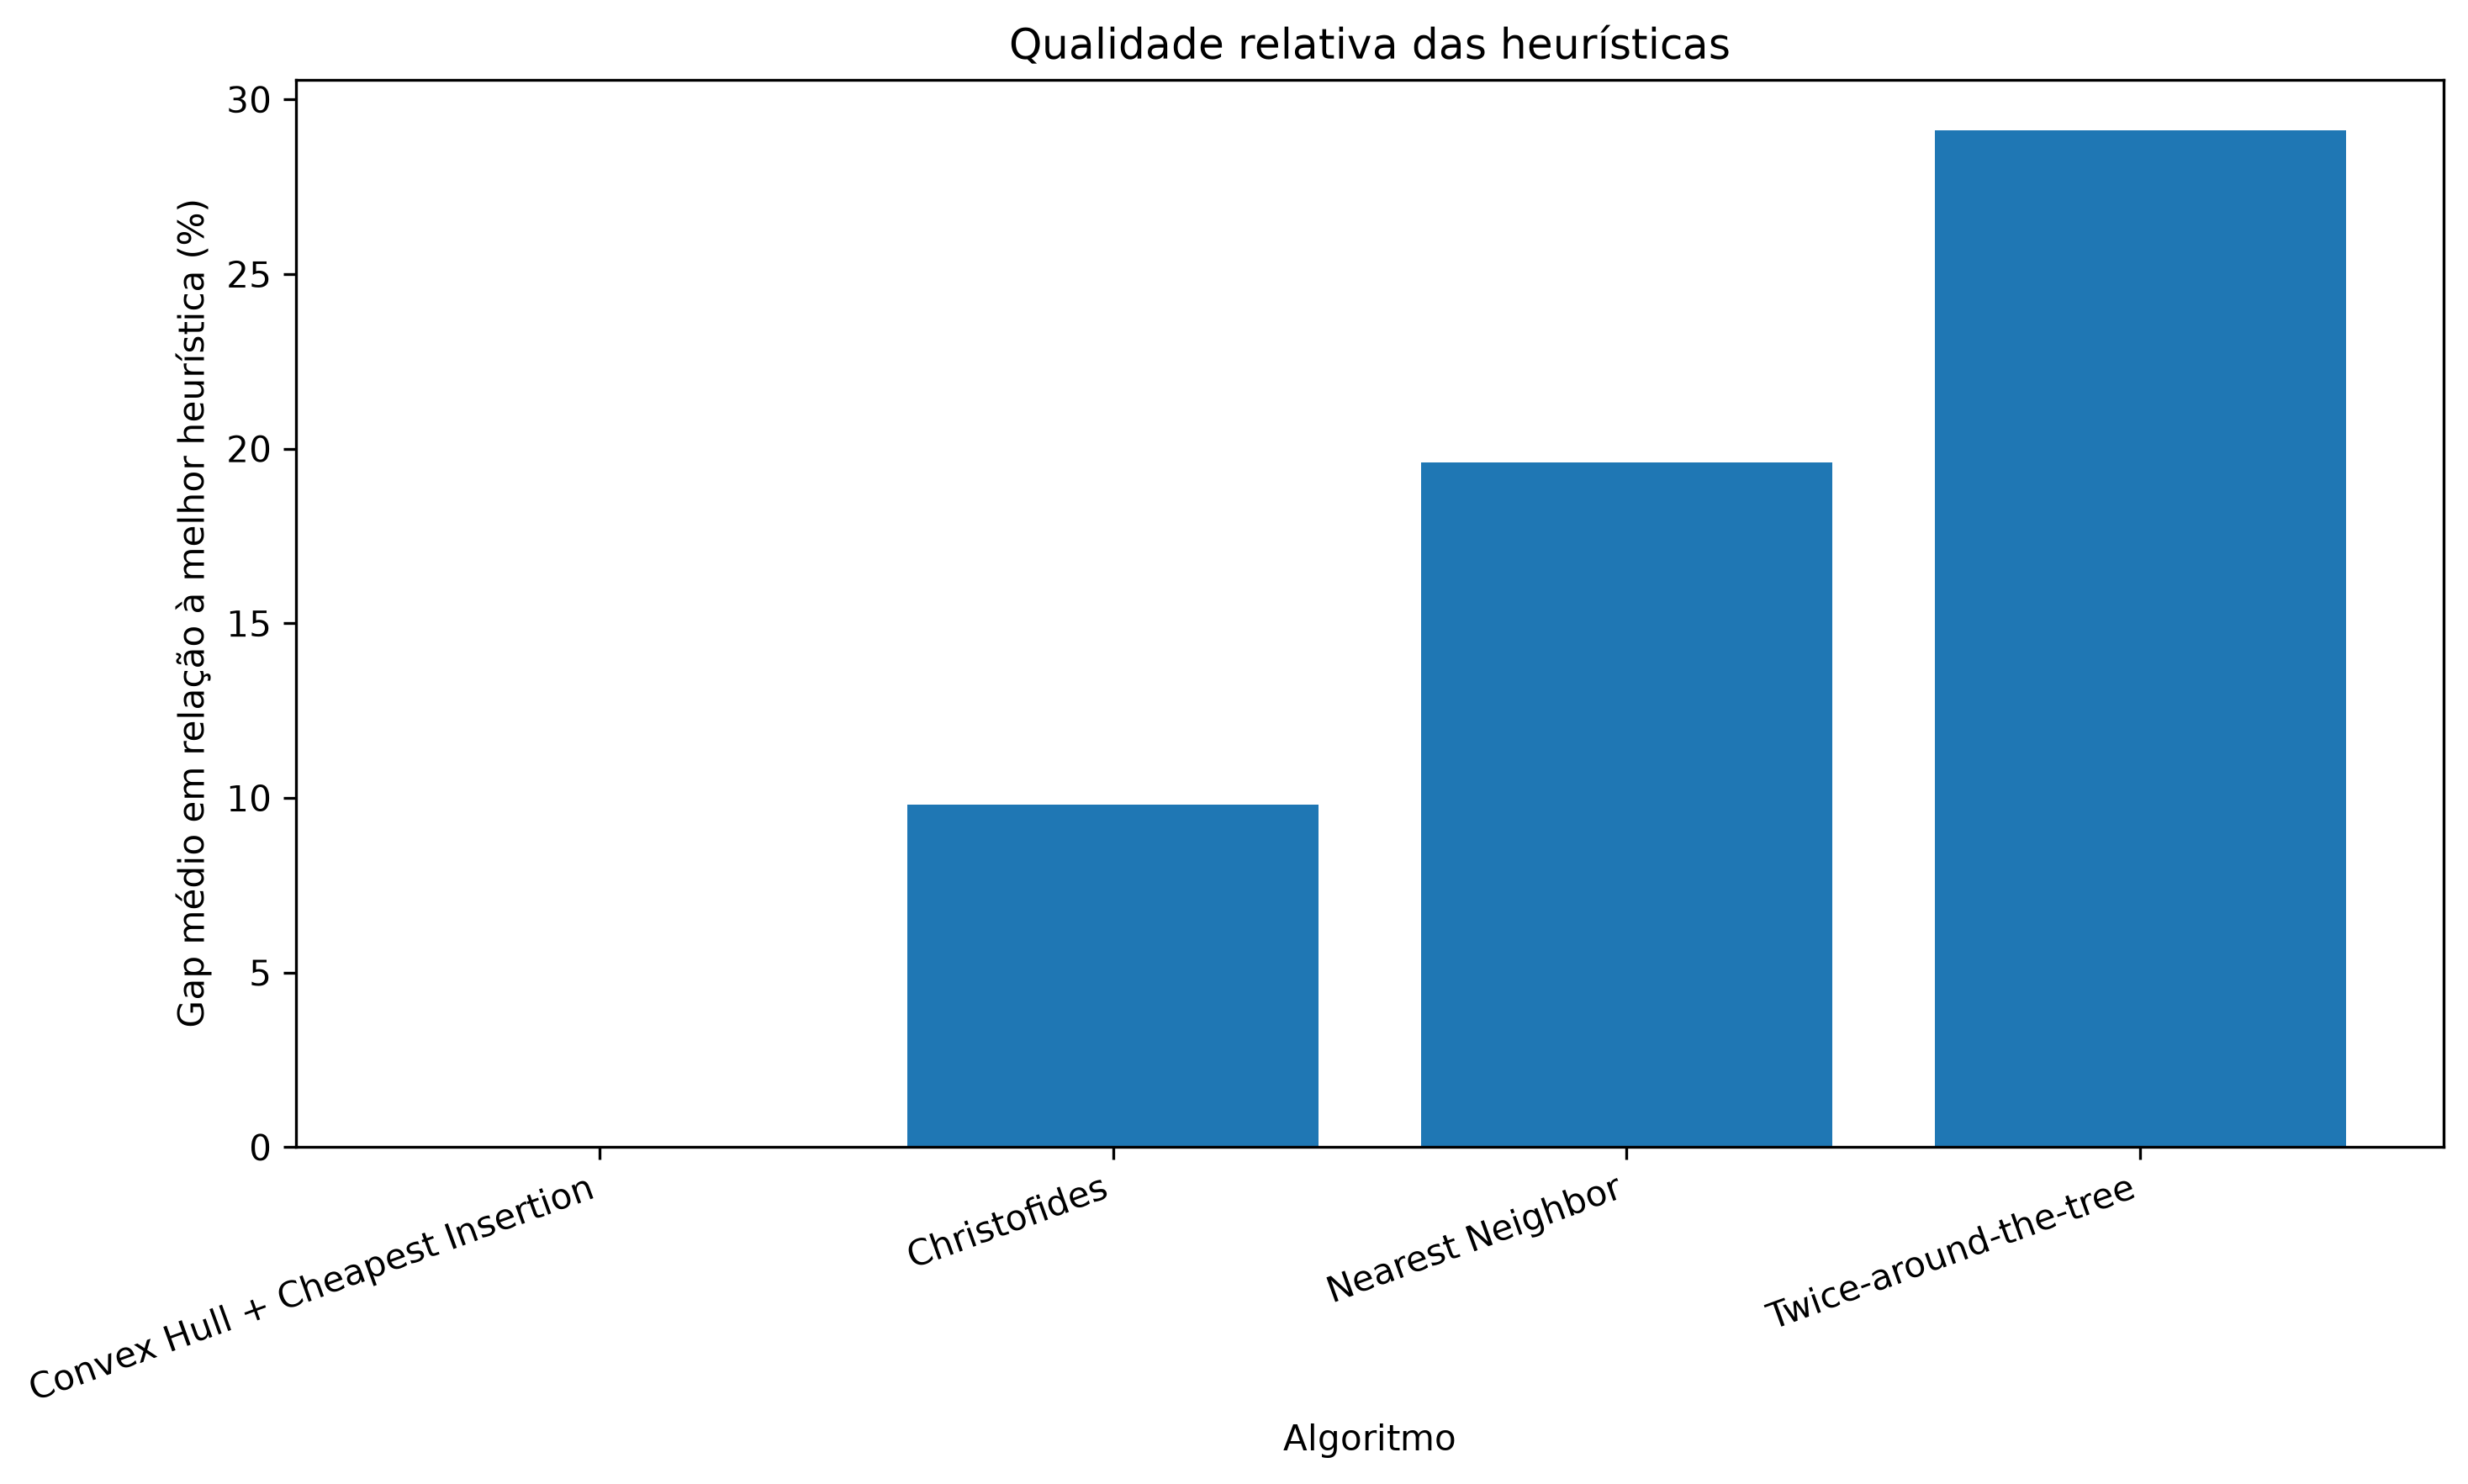
\includegraphics[width=0.82\textwidth]{figuras/qualidade_heuristicas.png}
\caption{Gap médio em relação à melhor heurística em cada instância.}
\label{fig:qualidade}
\end{figure}

\subsection{Comparação estatística}

Como os quatro métodos foram avaliados sobre as mesmas instâncias, foram utilizados testes pareados. O teste de Friedman apresentou estatística $38{,}52$ e $p=2{,}19\times10^{-8}$, indicando diferença global entre os algoritmos. Em seguida, foram realizadas comparações pareadas pelo teste de Wilcoxon, com correção de Holm para controlar o erro decorrente das múltiplas comparações.

\begin{table}[H]
\centering
\caption{Comparações de Wilcoxon com ajuste de Holm.}
\label{tab:wilcoxon}
\begin{tabular}{p{7.1cm}rr}
\toprule
Comparação & $p$ ajustado & Significativo\\
\midrule
Nearest Neighbor vs. Twice-around-the-tree & 0,05115 & Não\\
Nearest Neighbor vs. Christofides & 0,05115 & Não\\
Nearest Neighbor vs. Convex Hull + Cheapest Insertion & 0,00037 & Sim\\
Twice-around-the-tree vs. Christofides & 0,00037 & Sim\\
Twice-around-the-tree vs. Convex Hull + Cheapest Insertion & 0,00037 & Sim\\
Christofides vs. Convex Hull + Cheapest Insertion & 0,00037 & Sim\\
\bottomrule
\end{tabular}
\end{table}

Com nível de significância de 5\%, as diferenças entre Nearest Neighbor e Twice-around-the-tree, e entre Nearest Neighbor e Christofides, não permaneceram significativas após o ajuste de Holm. As demais comparações apresentaram diferenças estatisticamente significativas. A significância estatística não mede, por si só, a importância prática da diferença.

\subsection{Tempo de execução das heurísticas}

\begin{table}[H]
\centering
\caption{Tempos de execução das heurísticas (segundos).}
\label{tab:tempos}
\begin{tabular}{lrrrr}
\toprule
Heurística & Mediana & Média & Mínimo & Máximo\\
\midrule
Nearest Neighbor & 0,000037 & 0,000053 & 0,000007 & 0,000196\\
Twice-around-the-tree & 0,000160 & 0,000182 & 0,000033 & 0,000645\\
Christofides & 0,001938 & 0,003741 & 0,000350 & 0,017068\\
Convex Hull + Cheapest Insertion & 0,000460 & 0,001485 & 0,000036 & 0,009230\\
\bottomrule
\end{tabular}
\end{table}

Nearest Neighbor foi a heurística mais rápida em termos de tempo mediano. Convex Hull + Cheapest Insertion combinou o menor custo observado com tempo mediano inferior ao de Christofides. Christofides apresentou maior tempo mediano entre as quatro heurísticas, comportamento compatível com o custo adicional do matching de peso mínimo.

\begin{figure}[H]
\centering
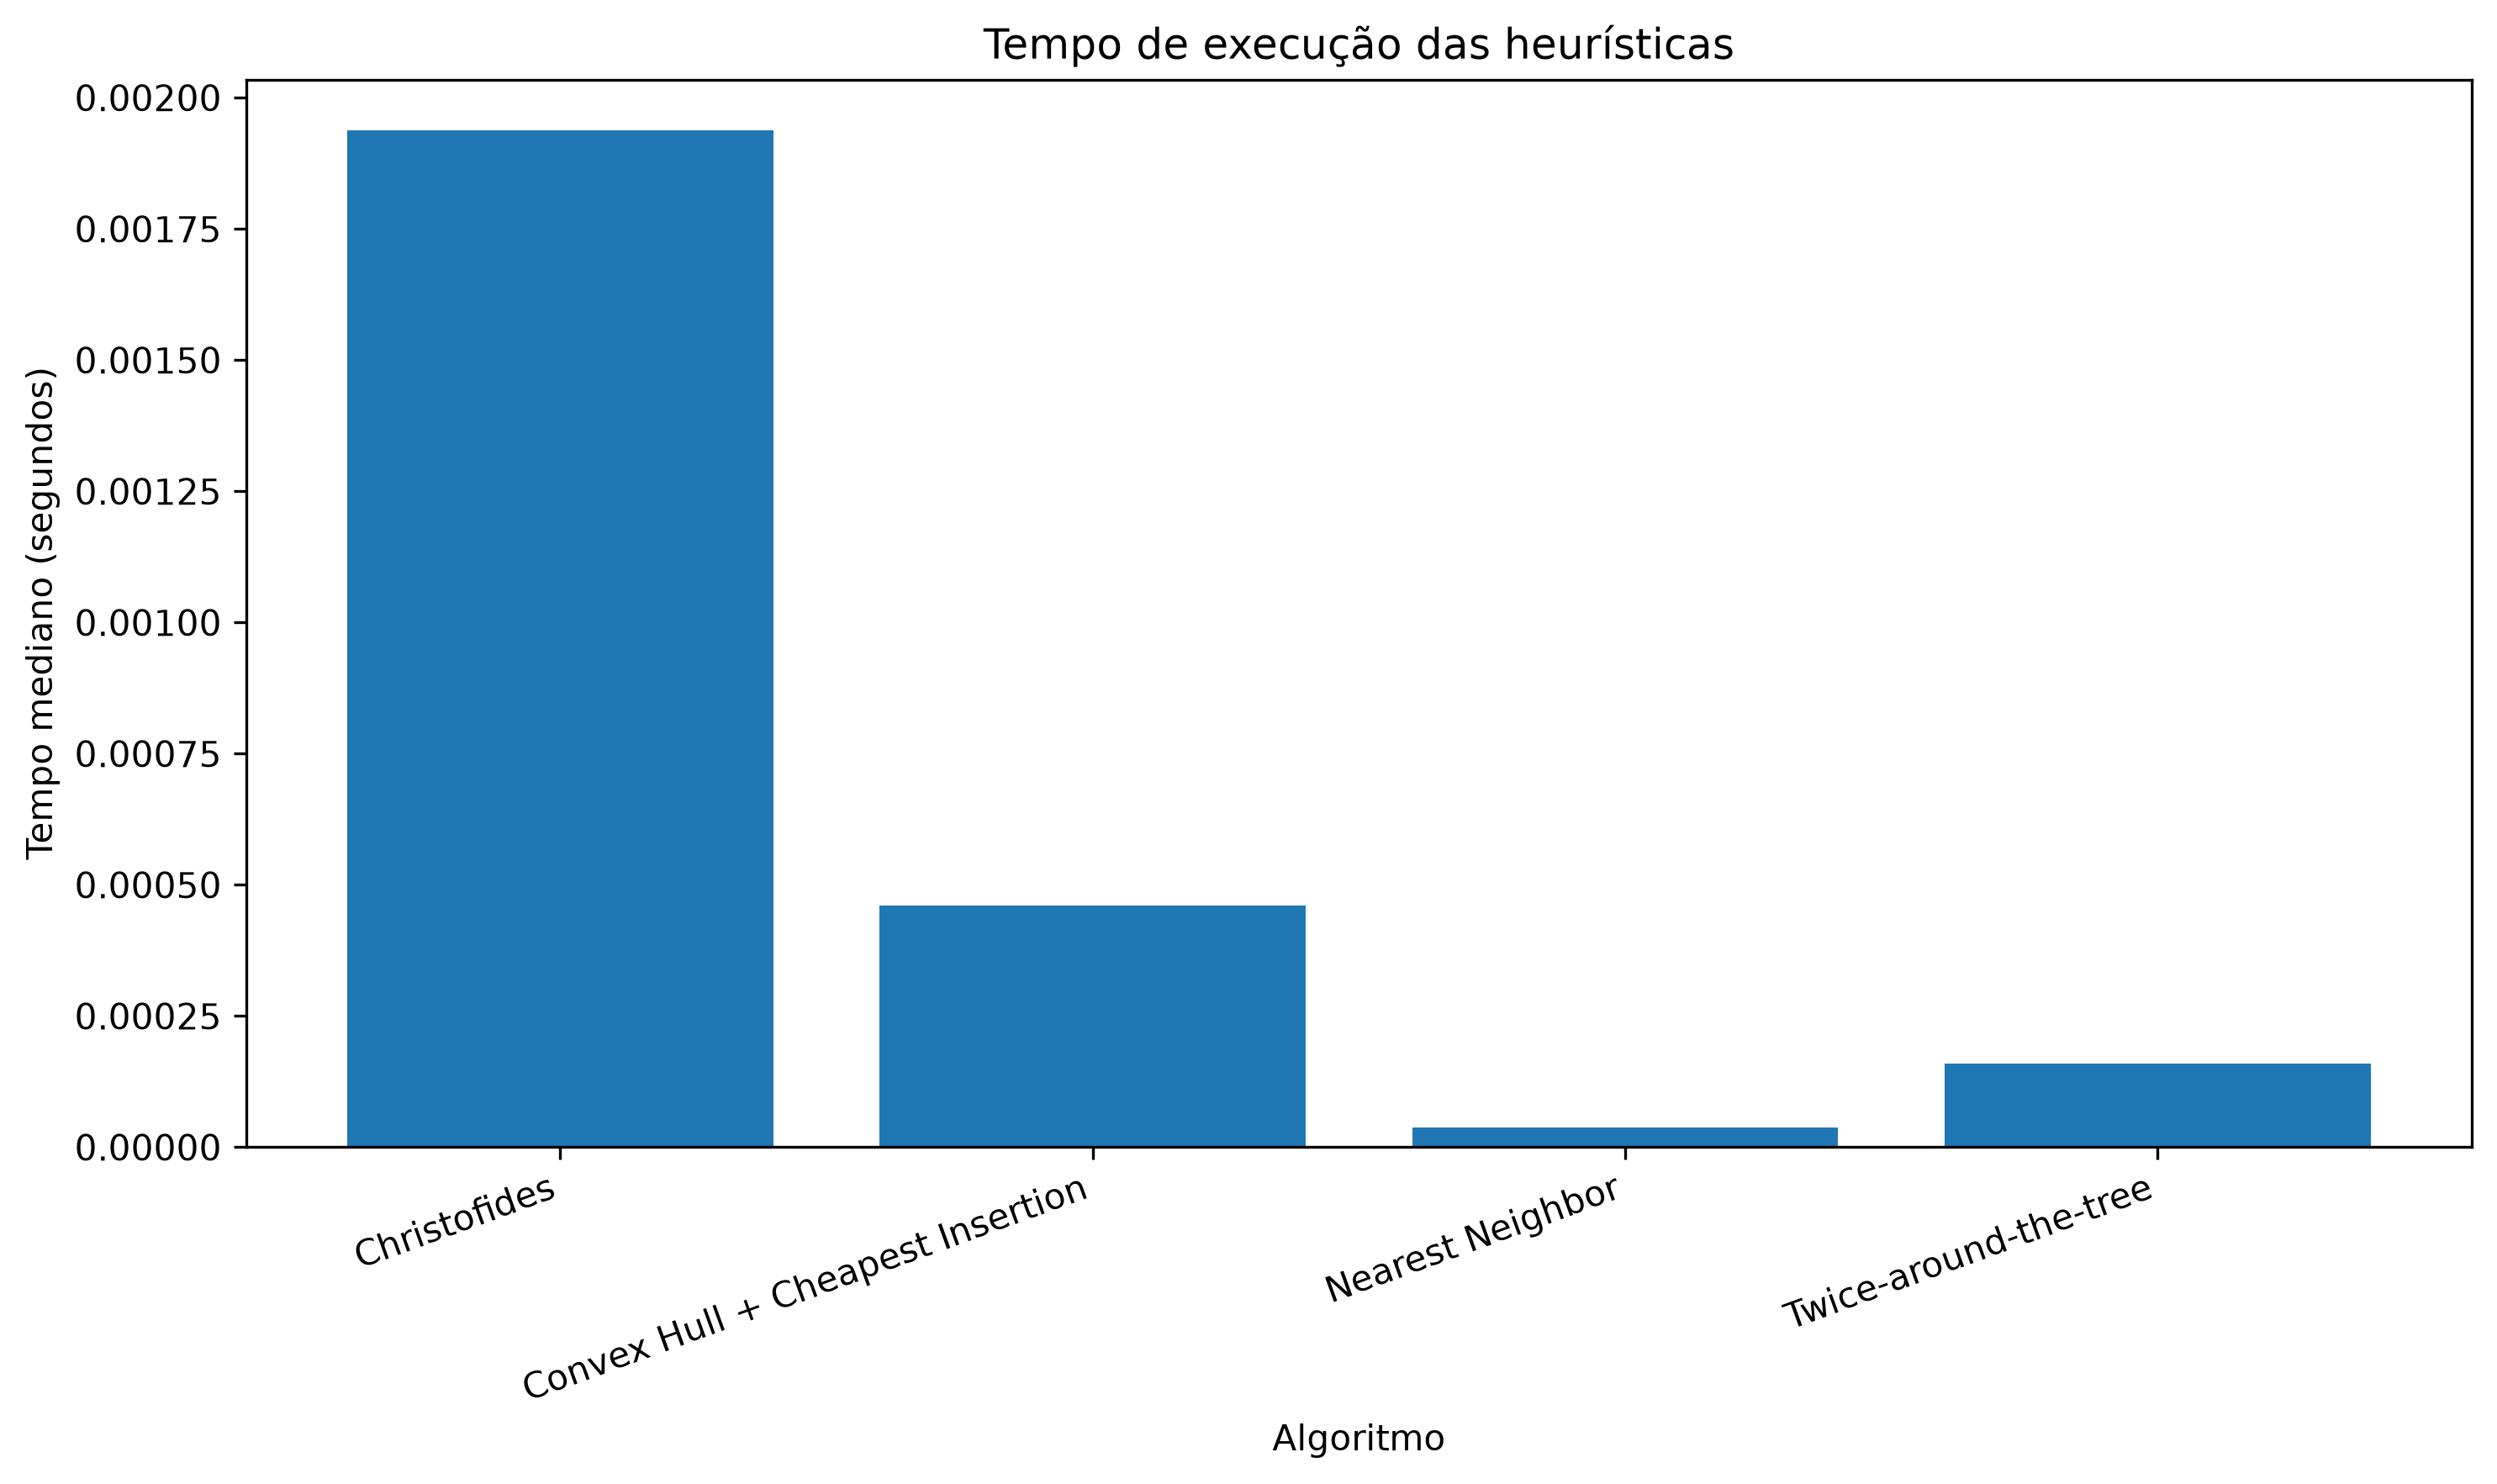
\includegraphics[width=0.82\textwidth]{figuras/tempos_heuristicas.png}
\caption{Tempo de execução das heurísticas.}
\label{fig:tempos}
\end{figure}

\subsection{Branch-and-Bound e estratégias de inicialização}

As 75 execuções oficiais resultaram em 50 conclusões com prova de otimalidade e 25 interrupções por tempo limite. Para cada uma das cinco estratégias, dez execuções terminaram com status \texttt{OTIMO} e cinco com \texttt{TIMEOUT}. Portanto, 66,7\% das execuções comprovaram a otimalidade e 33,3\% atingiram o limite configurado.

\begin{table}[H]
\centering
\caption{Situação das execuções oficiais de Branch-and-Bound.}
\label{tab:bb}
\begin{tabular}{lrrr}
\toprule
Estratégia & Ótimo provado & Timeout & Total\\
\midrule
Cold & 10 & 5 & 15\\
Nearest & 10 & 5 & 15\\
Convex Hull & 10 & 5 & 15\\
Twice & 10 & 5 & 15\\
Christofides & 10 & 5 & 15\\
\midrule
Total & 50 & 25 & 75\\
\bottomrule
\end{tabular}
\end{table}

A proporção idêntica de timeouts por estratégia não permite concluir, isoladamente, que as inicializações tenham desempenho equivalente. É necessário comparar os custos iniciais, os melhores custos obtidos, os tempos e os contadores de busca por instância, separando execuções ótimas de execuções interrompidas. Em particular, o custo final de uma execução \texttt{TIMEOUT} é um limite superior viável, não uma solução ótima certificada.

\subsection{Profiling de Christofides}

O profiling de Christofides foi realizado em cinco repetições por instância. No resumo agregado, o matching apresentou tempo mediano de 0,001847 s e memória mediana de 0,074766 MB, enquanto a AGM apresentou 0,000102 s e 0,003845 MB. O tempo mediano do algoritmo completo foi 0,002011 s e a memória mediana registrada foi 0,076948 MB.

Esses resultados apontam o matching como o componente dominante nas medições agregadas de tempo e memória. Essa observação é coerente com o fato de que o matching é uma etapa computacionalmente mais elaborada que a identificação dos vértices ímpares, a construção do multigrafo e a aplicação de atalhos. Os valores são específicos ao ambiente e às instâncias avaliadas.

\begin{figure}[H]
\centering
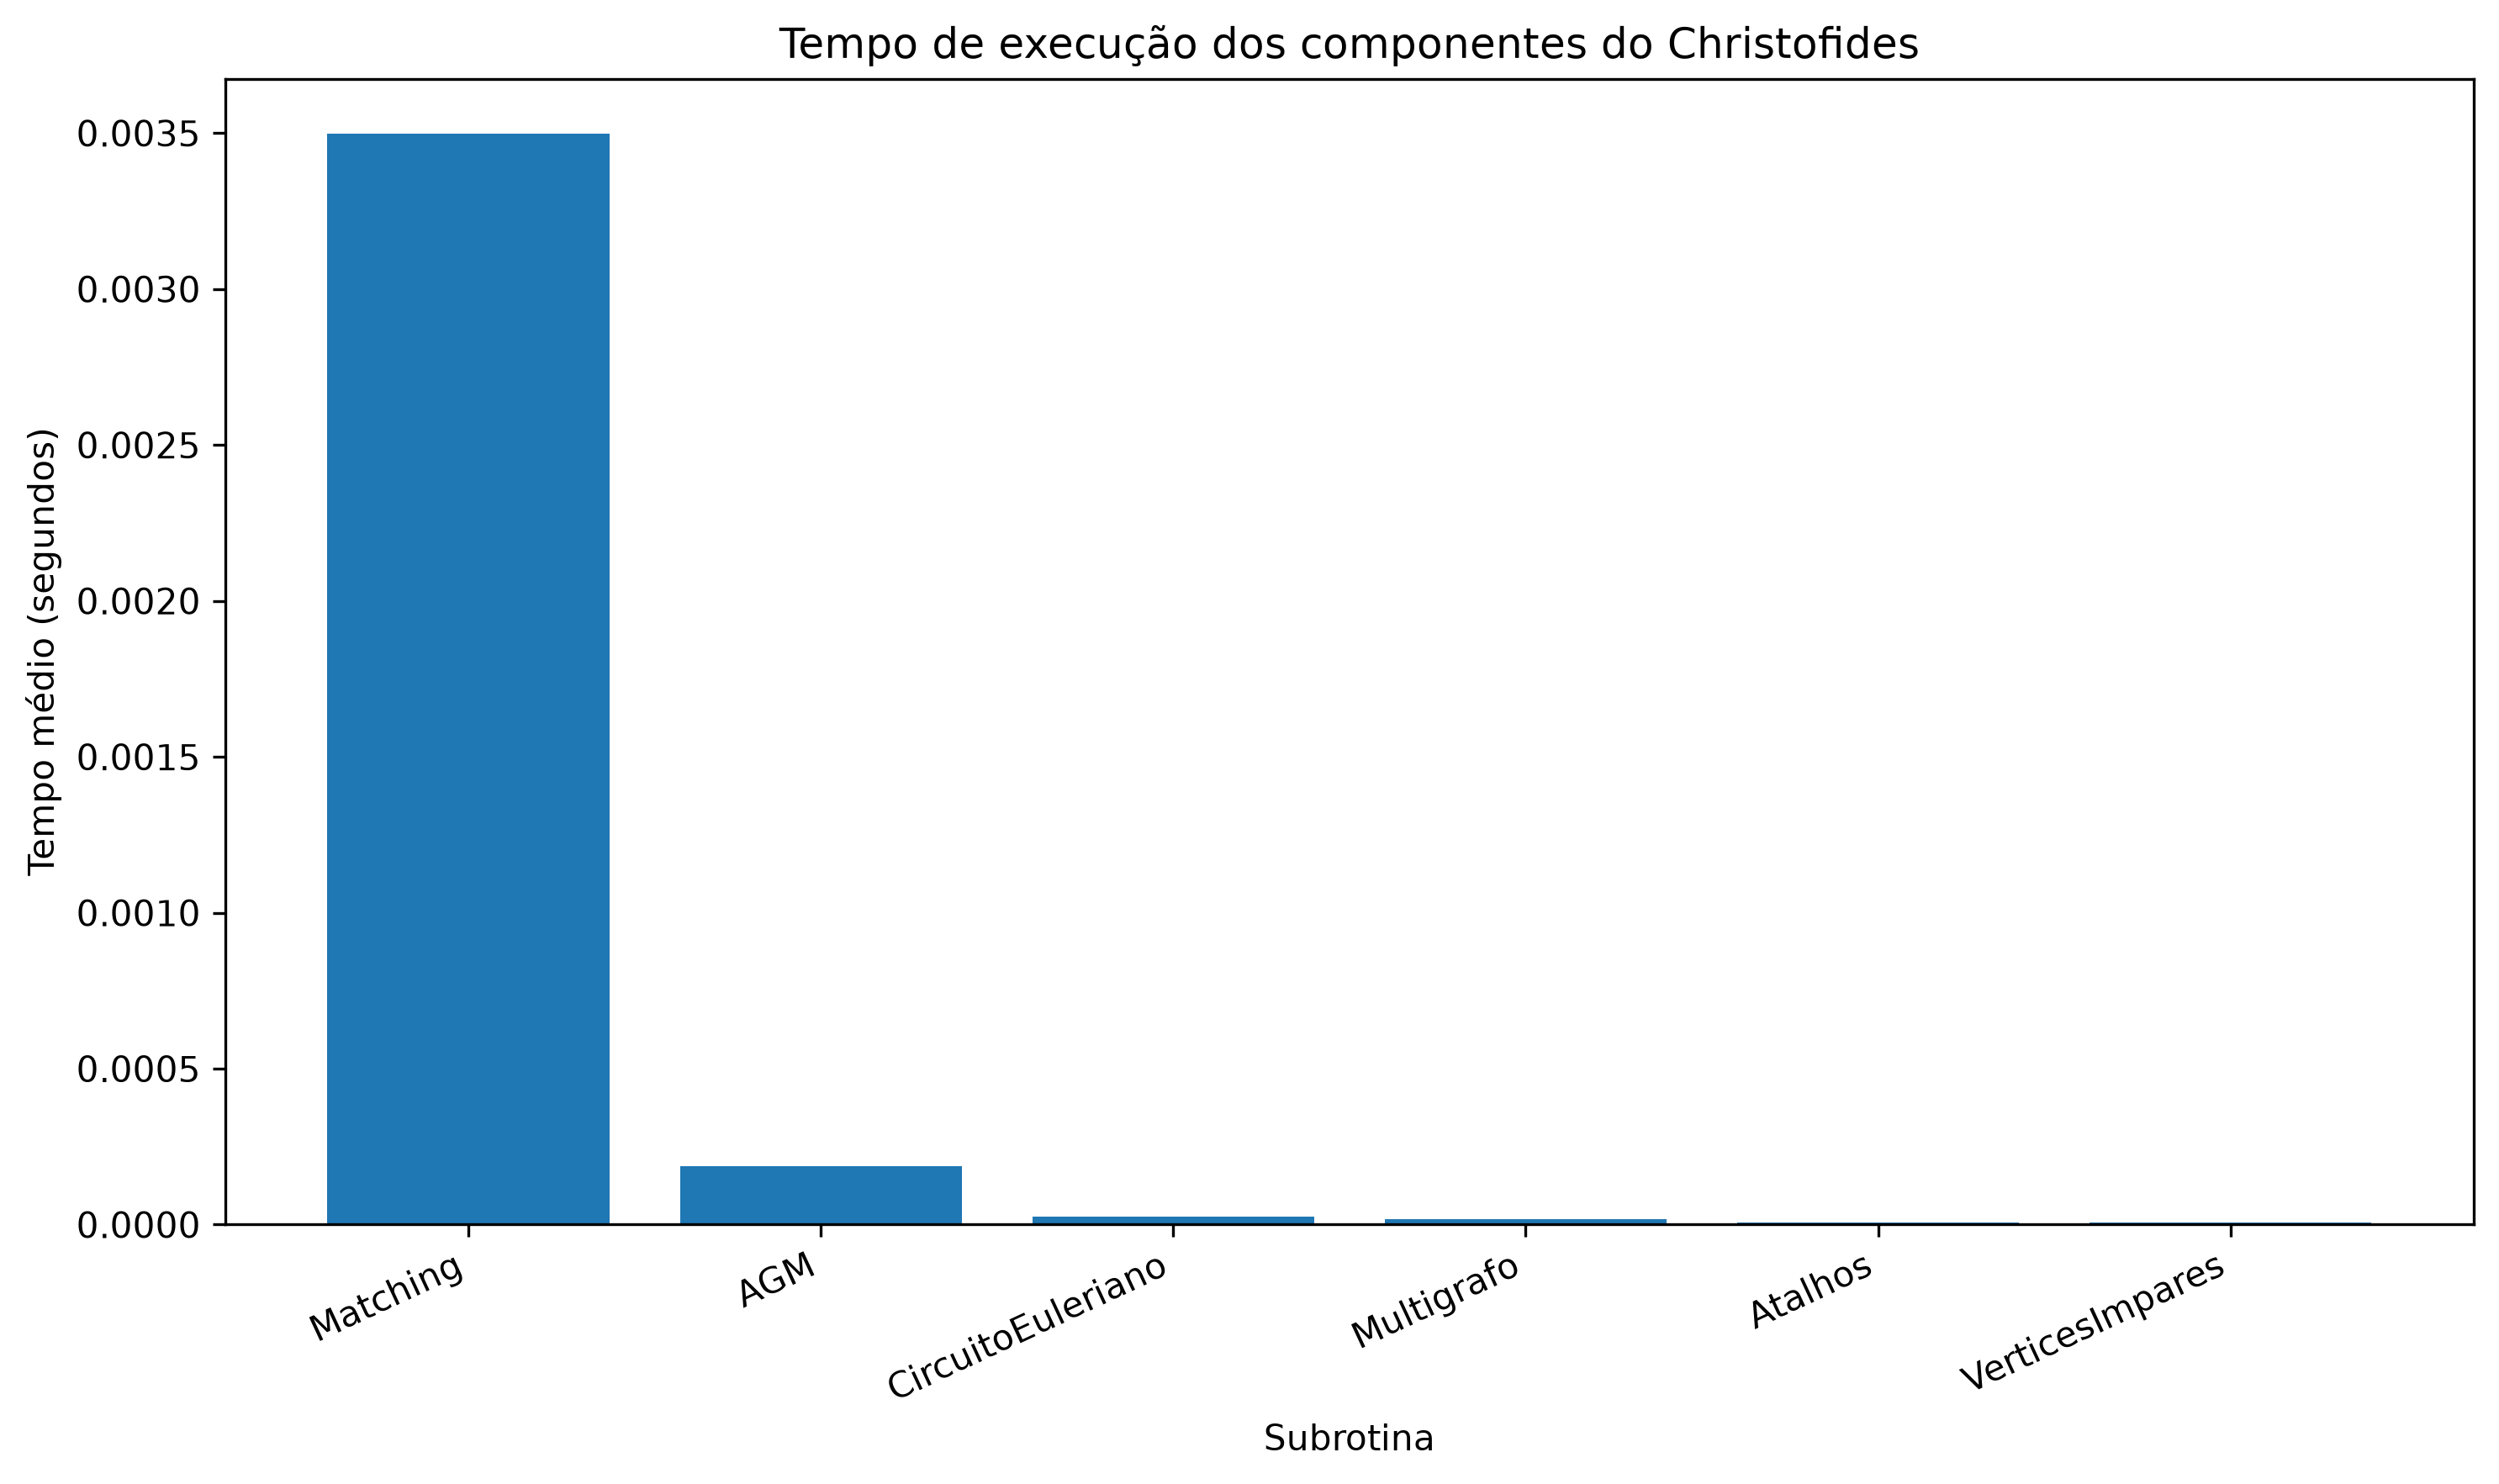
\includegraphics[width=0.82\textwidth]{figuras/profiling_componentes_tempos.png}
\caption{Tempos medianos dos componentes de Christofides.}
\label{fig:profilingtempo}
\end{figure}

\subsection{Características geométricas e escalabilidade}

Foram calculadas características como razão entre dimensões do retângulo envolvente (\textit{aspect ratio}), proporção de vértices no fecho convexo, entropia espacial, grau máximo da AGM e coeficiente de variação das distâncias ao vizinho mais próximo. As associações foram avaliadas por correlação de Spearman, com ajuste de Holm.

A associação mais consistente reportada foi entre a proporção de vértices no fecho convexo e o tempo de execução das heurísticas: os coeficientes de Spearman variaram de aproximadamente $-0{,}843$ a $-0{,}882$, com valores de $p$ ajustados inferiores a 0,003. Trata-se de uma associação negativa no conjunto observado: instâncias com maior proporção de vértices no fecho convexo tenderam a apresentar tempos menores. Como a amostra contém apenas 15 instâncias, e parte delas é derivada por seleção de vértices, esse resultado deve ser interpretado como exploratório, não causal.

Os modelos potência ajustados aos tempos das heurísticas apresentaram expoentes estimados de 1,63 para Nearest Neighbor, 1,61 para Twice-around-the-tree, 2,03 para Christofides e 2,83 para Convex Hull + Cheapest Insertion. Esses expoentes descrevem o ajuste empírico no intervalo de dimensões estudado; não constituem provas de complexidade assintótica e não devem ser extrapolados para dimensões muito maiores.

\begin{table}[H]
\centering
\caption{Expoentes dos modelos potência ajustados aos tempos.}
\label{tab:expoentes}
\begin{tabular}{lrr}
\toprule
Heurística & Expoente estimado & $R^2$\\
\midrule
Nearest Neighbor & 1,63 & 0,973\\
Twice-around-the-tree & 1,61 & 0,968\\
Christofides & 2,03 & 0,920\\
Convex Hull + Cheapest Insertion & 2,83 & 0,996\\
\bottomrule
\end{tabular}
\end{table}

\section{Conclusões}

A realização dos experimentos permitiu observar diferenças claras entre as abordagens avaliadas. Neste conjunto de instâncias, Convex Hull + Cheapest Insertion produziu as rotas de menor custo entre as quatro heurísticas, enquanto Nearest Neighbor foi a opção mais rápida. Christofides também apresentou bons resultados de qualidade, mas teve um custo de execução maior, principalmente por causa da etapa de matching.

Os testes estatísticos reforçaram que existem diferenças entre as heurísticas, mas também mostraram que nem todos os pares apresentaram diferença significativa depois da correção de Holm. Por isso, a comparação não deve se apoiar somente na ordem dos rankings: é necessário considerar os valores observados e o resultado dos testes.

No Branch-and-Bound, 50 das 75 execuções terminaram com prova de otimalidade, enquanto 25 chegaram ao limite de 1.800 segundos. Isso mostra que, mesmo com diferentes estratégias de inicialização, a busca exata pode exigir um esforço elevado. Também reforça a necessidade de separar os casos em que o ótimo foi comprovado daqueles em que o algoritmo apenas encontrou uma boa rota antes de ser interrompido.

O profiling mostrou que o matching foi a etapa mais custosa de Christofides nas medições realizadas. Já as análises geométricas e os modelos de escalabilidade ajudaram a levantar possíveis relações entre as características das instâncias e o desempenho, mas devem ser vistos como resultados exploratórios, considerando a quantidade e a composição do conjunto utilizado.

Como continuação, seria interessante ampliar o conjunto com instâncias independentes, realizar novas execuções em condições controladas e aprofundar a comparação das estratégias de inicialização do Branch-and-Bound. Também seria válido investigar com mais detalhes como o arredondamento das distâncias influencia as propriedades métricas utilizadas nas garantias teóricas dos algoritmos.

\section*{Referências}

\begin{thebibliography}{9}

\bibitem{lawler}
Lawler, E. L., Lenstra, J. K., Rinnooy Kan, A. H. G. and Shmoys, D. B. (eds.).
\newblock \textit{The Traveling Salesman Problem: A Guided Tour of Combinatorial Optimization}.
\newblock Wiley, 1985.

\bibitem{approx}
Christofides, N.
\newblock Worst-case analysis of a new heuristic for the travelling salesman problem.
\newblock Technical Report, Graduate School of Industrial Administration, Carnegie Mellon University, 1976.

\bibitem{tsplib}
Reinelt, G.
\newblock TSPLIB---A traveling salesman problem library.
\newblock \textit{ORSA Journal on Computing}, 3(4):376--384, 1991.

\bibitem{networkx}
Hagberg, A. A., Schult, D. A. and Swart, P. J.
\newblock Exploring network structure, dynamics, and function using NetworkX.
\newblock In \textit{Proceedings of the 7th Python in Science Conference}, 2008.

\end{thebibliography}

\end{document}